\documentclass[a4paper,12pt]{article}

\usepackage[81955]{MCMthesis}\problem{E}
\usepackage{palatino}
\usepackage{natbib}
\usepackage{graphicx}
\usepackage{listings}
\usepackage{float}
\usepackage{appendix}
\usepackage{threeparttable}


\setlength{\belowcaptionskip}{4pt}
\setlength{\abovecaptionskip}{4pt}

\usepackage{titlesec}
\usepackage{titletoc}
\setcounter{tocdepth}{2}

\titlecontents{section}[12mm]{\fontsize{12pt}{32pt}\selectfont \bf}{\contentslabel{2.5em}}{}{\titlerule*{.}\contentspage}
\titlecontents{subsection}[18mm]{\fontsize{12pt}{32pt}\selectfont \fs}{\contentslabel{3.3em}}{}{\titlerule*{.}\contentspage}



\usepackage[font=small,]{caption}
\def\abstractname{Summary}
\title{Research On the Ways Climate Change Influences Regional Fragility}  %Title

\begin{document}



%----------Summary----------
\begin{abstract}\footnotesize
Nowadays, it is widely realized that the problem brought by Climate Change is more of a social problem than a shallow environmental problem. Evidence has shown that it even has much to do with regional instability. Its assignable influence on each nation's development is indeed worth great amount of study. In this paper, our team focus on how to create a novel fragile state model in the light of Climate Change to find what humans can do to decrease fragility. 

\textbf{In task 1}, based on the gathered abundant data about fragility of states, 30 indicators are selected in our model. Based on Analytic Hierarchy Process (AHP) method and the Fragile States Index (FSI) defined by the Fund for Peace, we construct a new four-level indicator system and get the weight vector of indicators. The first level of the system has 1 indicator, the second level has 4 indicators, the third level has 12 indicators and the fourth level has 13 indicators to evaluate the fragile degree of the state. Moreover, the standard of the fragility, vulnerability and stability of the state is obtained through the threshold theory. In addition, we define the Climate Change Index which acts as an indirect contributor to increase fragility. 

\textbf{In task 2}, applying our model to Sudan, we find that Climate Change increases fragility of it via directly influencing the basic level indicators, thus reducing the values of 10 indicators shown by our model can decrease the fragility.

\textbf{In task 3}, China is selected to measure its fragility. Through stochastic processes, we simulate the future change of the indicator values, set the intensity of the changes in these indicators, and then classify it into three categories: low, middle and high. Next we measure China's fragility in each scenario and define the tipping point by sensitivity method. If the fragility reaches the point, China will be more fragile. In our model, better performance is shown versus the FSI model.

\textbf{In task 4}, we propose interventions based on our model which shows that five factors impacting fragility are most relevant to Climate Change. Then we analyze methods and data from literature, calculating costs to maintain each factor at the normal level, and classify countries into two categories: stable and unstable. By dynamic programming algorithm, the minimum total costs to maintain each impact factor are predicted.

\textbf{In task 5}, we evaluate the applicability of our model and find that although it has universality to a certain extent, it can be modified to better work on "states" of various sizes. Thus we define the risk parameter to be taken as a coefficient into the model, and select a city and a continent to analyze sensitivity, finding that the original model is effectively improved.

Finally, we analyze the strengths and weaknesses of the proposed models in this paper. The research can be also applied for studies of what humans can do to decrease a state's fragility relevant to Climate Change.



\end{abstract}

\maketitle
\thispagestyle{empty}

\newpage
\setcounter{tocdepth}{3}
\tableofcontents
\thispagestyle{empty}
\newpage

\setlength\parskip{0.8\baselineskip}
\setcounter{page}{1}
\pagestyle{fancy}

\section{Introduction}
\subsection{Background}

The effects of Climate Change, such as increased droughts, flooding and sea level rise, have already appealed to much caution. Many people believe that the Climate Change is not only an environmental problem but increasingly becomes a threat to social development. Climate changes especially the ones that bring natural disasters will bring much pain to people living in that region. And the net damage costs of Climate Change are likely to be unbearable. Many of the Climate Change effects will alter the way humans live, and may have the potential to cause the weakening and breakdown of social and governmental structures. Consequently, destabilized governments could result in fragile states.
\paragraph{A country's fragility}
A fragile state is one where the state government is not able to, or chooses not to, provide the basic essentials to its people. According to the authentic Fragile State Index, the country's fragility is determined by 12 items including three cohesion indicators, three economics indicators, three political indicators and three social and cross-cutting indicators. However, Climate Change, as has been discussed, is also an important contributor to contemporary nation's fragility but was neglected by the Fund for Peace in measuring a country's fragility. To find out the accurate relationship between a country's Climate Change and its fragility, we refer to many references to search for rules which could lead to a distinct function between a country's system and the Climate Change index. In this paper, we develop a model that can determine a country's fragility and simultaneously measure the impacts of the Climate Change.
\subsection{Problem Statement and Analysis}

Since Climate Change is essential to a nation's stability, it is significant to structure the mechanism about how does the Climate Change influence the value of fragility of a nation. In this way of thinking, we must find quantitative indicators to measure the region's Climate Change and its fragility. Through piles of documents, we decide to use AHP method to describe the relationship between Climate Change and its fragility. Further, two specific countries are selected to evaluate the fragility of them, with and without the influences of Climate Change. Moreover, we have to propose feasible plans to help the country become more stable. At last, we need to explain the applicability of our model and modify our model to make it more common.   

\section{Methodology}

\subsection{Climate Change Index}
\label{sec:document-classes}

To measure the Climate Change, we define the Climate Change Index. Considering the availability of data and the relevance to climate conditions, the index takes into account a temperature measure and a precipitation measure \citep{alexander2006global}.

 Since the Climate Change Index is for the fragility model, the results of which are expected to be presented in years, we seek to give yearly data of the two measures. However, we can only get the data of monthly mean maximum temperature (The average daily maximum temperature over a month), monthly mean minimum temperature (The average daily minimum temperature over a month) and monthly mean precipitation. So we take average of the monthly data to obtain the yearly data.

 Thus, we define the change rate of yearly mean maximum temperature, the change rate of yearly mean minimum temperature and the change rate of yearly mean precipitation. Since we are concerned about the magnitude of change rather than the direction, the absolute value is taken.
\begin{equation}
\label{eq1}
C_{temperature~max}=\left|\frac{{temperature~max}_n-{temperature~max}_{n-1}}{{temperature~max}_{n-1}}\right|
\end{equation}
\begin{equation}
\label{eq2}
C_{temperature~min}=\left|\frac{{temperature~min}_n-{temperature~min}_{n-1}}{{temperature~min}_{n-1}}\right|
\end{equation}
\begin{equation}
\label{eq3}
C_{precipitation~mean}=\left|\frac{{precipitation~mean}_n-{precipitation~mean}_{n-1}}{{precipitation~mean}_{n-1}}\right|
\end{equation}
\noindent{Where:}

\qquad${temperature~max}_n$ = mean maximum temperature of the Nth year

\qquad${temperature~max}_{n-1}$ = mean maximum temperature of the (N-1)th year

\qquad$C_{temperature~max}$ = change rate of mean maximum temperature of the Nth year

\qquad And the rest can be done in the same manner.
\\


From the above, the Climate Change Index can be defined as follows:
\begin{equation}
\label{eq4}
CCI=C_{temperature~max}+	C_{temperature~min}+C_{precipitation~mean}
\end{equation}
(An additive form is chosen instead of a multiplicative form, because if a single indicator is very small, the change of CCI will converge towards zero; a linear form is chosen instead of a nonlinear form for ease of calculation. )

The higher the three change rates are, the higher CCI is, indicating that the country has undergone a great Climate Change this year.


\subsection{Fragile National Index Model}
\label{sec:document-classes}

To measure the national vulnerabilities, we define Fragile National Index (FNI) based on the Fragile States Index (FSI) defined by the Fund for Peace. FNI includes four major items - cohesion, economic, political and social.




This model outputs a Fragile National Index (FNI) value that ranges across a traditional grading system of 0-120 (where 120 is the highest possible level of Smart Growth). This FNI value is the sum of scores from the four items mentioned previously.

\begin{equation}
FNI=Cohesion+Economic+Political+Social
\end{equation}

Each of the sub-items is assumed to have the same importance, so each is weighed evenly in the above equation. Each sub-item can have an output between the range of 0-10, meaning the highest possible FNI would have a rating of 10 for each sub-item, which then sums to 120.

The 12 items which determine a country's fragility are divided into four aspects. After reading many references and careful discussion, we believe that the change of climate is mainly through an indirect way to impact on a nation's fragility. Usually, the Climate Change will first have effect on the country's natural resources and in turn influence its economy, population density, relationship between environment and citizenry, etc. In the following, we will demonstrate the relationship between Climate Change and the twelve items linked to a country's fragility in every aspect at length. 

From the cohesion aspect, security apparatus, factionalized elites and group grievance are considered. The authentic Fragile State Index tells us that security apparatus includes the monopoly on the use of force, relationship between security and citizenry and force and arms.

From the above, the Cohesion can be calculated as follows:
\begin{equation}
Cohesion=Security\;Apparatus+Factionalized\;Elites+Groups\;Grievance
\end{equation}
where:
\begin{equation}
\label{eq7}
\begin{split}
Security\;Apparatus&=Monopoly\;on\;the\;use\;of\;Force\\&+Relationship\;between\;Security\;and\;Citizenry\;\\ &+\;Force\;and\;Arms
\end{split}
\end{equation}

However, simply adding up these factors to obtain the security apparatus value seems not rigorous. That is a very definite possibility that different factors put different weight on the output \citep{saaty2008decision}. So we adopt the method of Analytic Hierarchy Process (AHP), which makes an organic combination of qualitative analysis and quantitative analysis, finding the relative priority weight. The distinction of this method lies in its excellent performance to quantify a complex qualitative problem, and the definition of security apparatus happens to be a complex qualitative problem. To obtain a quantitative evaluation scheme, it is appropriate to apply AHP.

The steps of AHP are as follows.

\paragraph{Expert's ranking} We distributed questionnaires among experts to ask for advice, collecting their opinions of the rank of indicators' importance. Since the objective was to evaluate security apparatus, these experts' research fields varied from defense science, technology information science, military science, etc, thus having great representativeness. The questionnaires were sent by e-mail, 20 copies were handed out and 20 were taken back, among which 20 were valid. The data of each expert's mark on each indicator's importance was processed by Excel to calculate the average score, providing reliable reference for the importance ranking of indicators. 

\paragraph{Weight's calculation and consistency check} With the data of indicators' importance ranking, we constructed a comparison matrix, the elements in which reflect the relative importance of the indicators. Based on the matrix, we calculated the weight of each indicator based on C++ (\ref{prog}). When the order of the matrix $n>2$, it is often difficult to construct one that satisfies the consistency, but there should be an upper limit where the deviation can be. So it is indispensable to identify whether or not the matrix can be accepted, which is the connotation of the consistency check.


Via AHP, equation \eqref{eq7} can be improved as follows (values of weight are rounded up to 2 decimal places):
\begin{equation}
\begin{split}
Security\;Apparatus&=0.25*Monopoly\;on\;the\;use\;of\;Force\\&+0.5*Relationship\;between\;Security\;and\;Citizenry\;\\ &+\;0.75*Force\;and\;Arms
\end{split}
\end{equation}

 According to an increasingly widespread view, the country's security apparatus is frequently assumed to be connected with the Climate Change. Ole Magnus Theisen conducted a scarcity model of conflict, assuming that if Climate Change results in a reduction in essential resources for livelihood, such as food or water, those affected by the increasing scarcity may start fighting over the remaining resources \citep{Theisen2013Is}. It means that Climate Change risking people's living will increase the use of force, making the country's stability fall down. Additionally, If Climate Change results in reduced precipitation and higher temperature that jointly cause droughts, and reduced access to the natural capital that sustains livelihoods, poverty will be more widespread and the potential for conflict greater \citep{Gleditsch2014Whither}. In personal level, Anderson's research \citep{Anderson2001Heat} suggests that hot temperatures will lead to violent personal crimes and riots. 
 
 In sum, Climate Change can affect a country's security apparatus through changing the use of force and relationship between security and citizenry. The worse the Climate Change is, the worse the security apparatus will be, the more fragile the country will be. Taking into account that CCI turns out to be a decimal, we consider (CCI+1) as the contributor to multiply the indicator of monopoly on the use of force and relationship between security and citizenry:

\begin{equation}
\label{eq9}
\begin{split}
Security\;Apparatus&=0.25*Monopoly\;on\;the\;use\;of\;Force*(CCI+1)\\&+0.5*Relationship\;between\;Security\;and\;Citizenry*(CCI+1)\\ &+\;0.75*Force\;and\;Arms
\end{split}
\end{equation}

In fact, the elements contained in the equation also have their quantitative standards and they can be evaluated as shown in the appendix(Appendices Figure \ref{fig6}).

The economic indicators include economic decline, uneven economic development and human flight and brain drain. The economic decline is usually defined by the decrease of DPI (Disposable Personal Income), GDP (Gross Domestic Production) and the increase of unemployment rate. And the uneven economic development is linked with group economic divide, perception of inequality and economic opportunity. Using AHP described above, the weight of each indicator can be determined as follows:
\begin{equation}
\begin{split}
Economic\;Decline&=0.39*Decrease\;of\;DPI\\&+0.5*Decrease\;of\;GDP\\ &+0.61*Increase\;of\;unemployment\;rate
\end{split}
\end{equation}
\begin{equation}
\begin{split}
Uneven\;Economic\;Development&=0.79*Group\;Economic\;Divide\\&+0.34*Perception\;Of\;Inequality\\&+0.34*Economic\;Opportunity
\end{split}
\end{equation}

A great deal of research provides evidence for the influence of Climate Change on a nation's economy. Climate change threatens the economy of the nation through increased flooding and storm damage, climate-driven changes in crop yields, disruptions in labor productivity, crime, and public health and heat-related strains on energy systems \citep{houser2015economic}. So the DPI and GDP will naturally decrease but the  unemployment rate will increase. Furthermore, the Climate Change may expand the gap between the poor and the wealth. Because the Climate Change will first damage a nation's natural resources and agriculture, forcing farmers lose their source of finance and giving the wealth chances to press on the poor \citep{Schwartz2003An}. In this condition, Climate Change increases the group economic divide and reduces the economic opportunity.

\begin{equation}
\label{eq12}
\begin{split}
Economic\;Decline&=0.39*Decrease\;of\;DPI*(CCI+1)\\&+0.5*Decrease\;of\;GDP*(CCI+1)\\ &+0.61*Increase\;of\;unemployment\;rate*(CCI+1)
\end{split}
\end{equation}
\begin{equation}
\label{eq13}
\begin{split}
Uneven\;Economic\;Development&=0.79*Group\;Economic\;Divide*(CCI+1)\\&+0.34*Perception\;Of\;Inequality\\&+0.34*Economic\;Oppotunity*(CCI+1)
\end{split}
\end{equation}

Finally, the social and cross-cutting indicators include demographic pressures, refugee and IDPs and external invention. Take demographic pressures for detailed analysis. According to Fund for Peace description, demographic pressures are determined by population density and resource per capital. The refugee and IDPs indicator can be measured by a nation's relief slack and the number of its refugees. Using AHP described above, each indicator in these two equations happens to have the same weight:
\begin{equation}
%\begin{split}
Demographic\;pressures=Population\;Density+resource\;per\;capital
%\end{split}
\end{equation}
\begin{equation}
%\begin{split}
Refugee\;and\;IDPs=Relief\;Slack+Number\;of\;its\;refugees
%\end{split}
\end{equation}

About one-half of the world's population is tied directly to the land. However, nowadays, environmental stress is playing an ever-growing role in the conflicts between population and land. Drought, desertification, deforestation, and soil erosion and exhaustion leave the land afford fewer and fewer people\\\citep{Krakowka2012Modeling}. Such condition aggravates the lack of resources, thus more and more refugee and IDPs are springing up. So the Climate Change can result in more pressure between people and land, bringing more refugee and IDPs. It means that population density, the decline of resources per capital and the number of refugees and IDPs will be increased because of the worse climate. These can be concluded as:

\begin{equation}
\label{eq16}
\begin{split}
Demographic\;pressures&=Population\;Density*(CCI+1)\\ &+resource\;per\;capital*(CCI+1)
\end{split}
\end{equation}
\begin{equation}
\label{eq17}
%\begin{split}
Refugee\;and\;IDPs=Relief\;Slack+Number\;of\;its\;refugees*(CCI+1)
%\end{split}
\end{equation}

\begin{figure} [H]
\centering
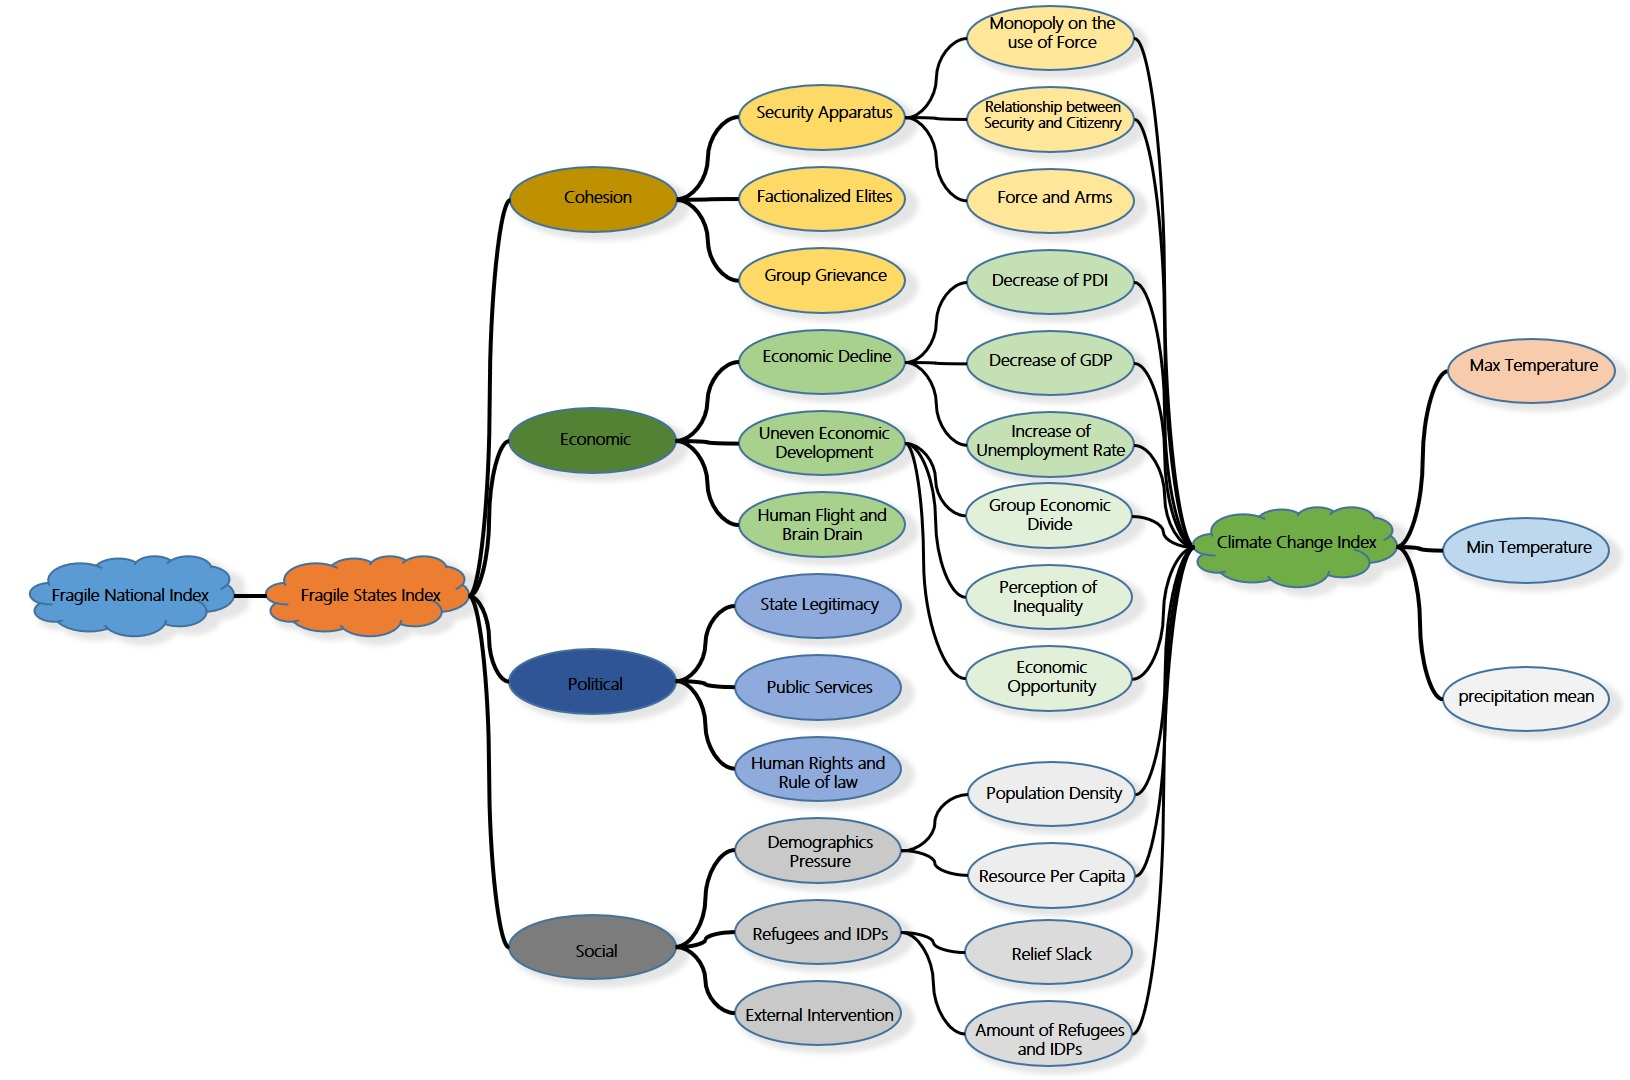
\includegraphics[width=\textwidth]{All.jpg}
\caption{The FNI indicator system diagram}%%%%%%%%%%%%%%%%%%%%%%%%%%%%%%%%%%%%%改名字!
\end{figure}

\subsection{Threshold}
\label{sec23}

To identify when a state is fragile, vulnerable, or stable, we introduce the threshold theory. The combination of threshold theory and index measurement, on the one hand, makes up for the shortcomings of the single quantitative method, on the other hand, combines stakeholder feedback, making the result more policy guiding. For example, The concept of the limited adaptability of the system is emphasized by \cite{polsky2007building}, followed by the question 'What is limited?', which requires the intervention of threshold theory, determining the threshold range of adaptability in comprehensive assessment based on actual situation and feedback. The adaptability of the evaluation unit below the minimum threshold or higher than the maximum threshold is too weak or too strong, indicating that the state is fragile or stable, the grey area between them is vulnerable.

According to the fragile national model described above, we can obtain the FNI values of the countries with the data of indicators, on which the Climate Change Index has effects. A graph of the results can be plotted as follows:


\begin{figure} [H]
\centering
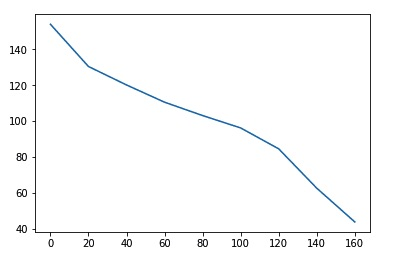
\includegraphics[width=\textwidth]{3.jpg}
\caption{The fitting curve of the countries' FNI}
\label{fig1}
\end{figure}


By analyzing the graph, we can find two extreme cases: lower than 87 (keep integer) or higher than 128 (keep integer). According to our model, 59 countries stand in the former group, 26 countries stand in the other, with the rest in the grey area between them. Thus, the thresholds have been distinguished as follows:

\begin{figure} [H]
\centering
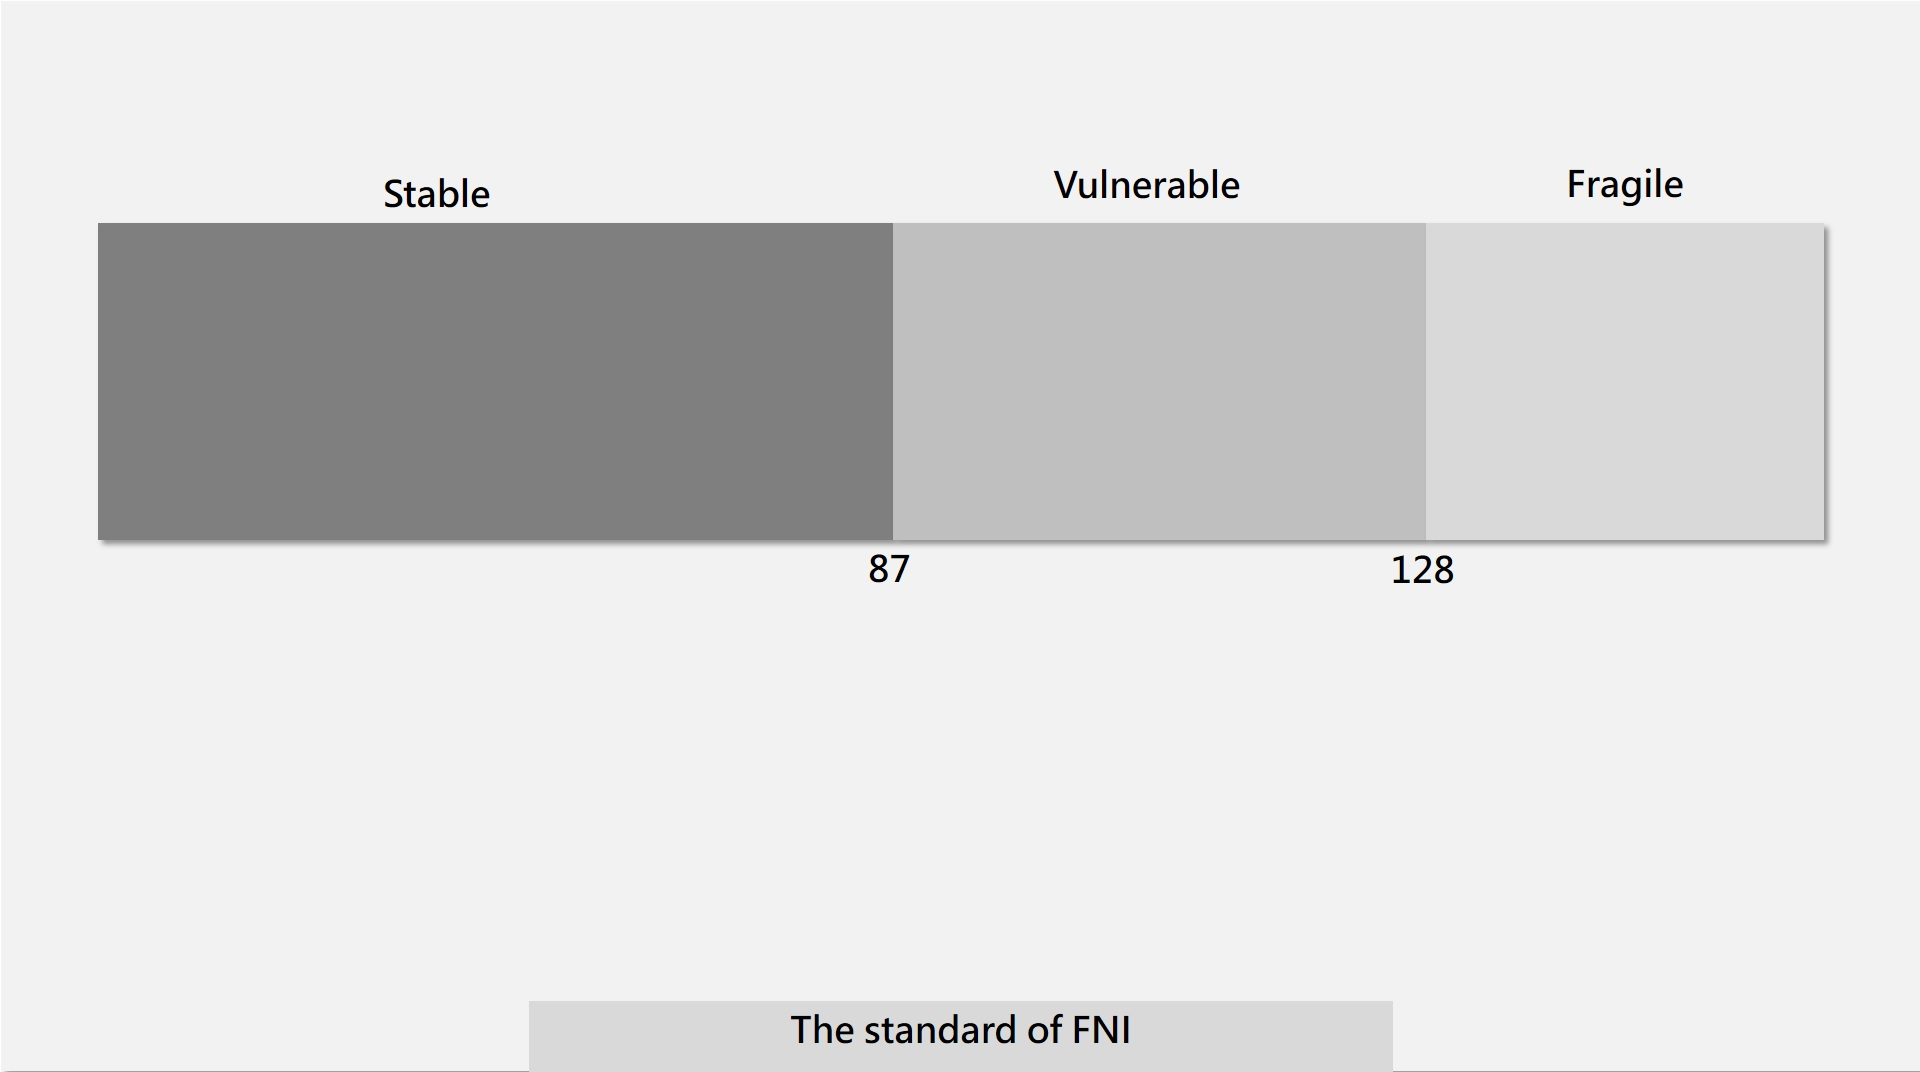
\includegraphics[width=15cm]{2.jpg}
\caption{The standard of the fragility, vulnerability and stability of the state}
\label{fig2}
\end{figure}

Although the thresholds are derived from the 2017 model, we can reasonably apply this identification system to other years, since each year's FNI value of a specific country has little difference.


\section{Model Applying}
In this section, we decide to select Sudan and China to testify our model. Sudan is chosen because it is one of the top 10 most fragile states as determined by the Fragile State Index. We are going to demonstrate how Climate Change may have increased fragility of Sudan and use our model to show in what way the state may be less fragile without these effects. China, with a middle rank among the states all around the world, is a good example to show in what way and when Climate Change may push it to become more fragile. Through the model application of China, we will also define a tipping point and predict when a country may reach it.
\subsection{Model Application in Sudan}
Our FNI model inherits that a nation's fragility is related to its 12 items given by the FSI. However, not limited to the FSI model, we further conduct study finding that some items are directly or indirectly connected with the nation's Climate Change and try to figure out the definite relationship between a nation's Climate Change and its stability. It's very important to note that Climate Change has a complex inner relationship with a country's 12 basic items which can measure the country's fragility. Considering the variety of climate and the complicated inner influence mechanism, the FNI model is more comprehensive and can better measure a nation's fragility.
Compared with primitive FSI model, in FNI, CCI is a contributor added into the improved model. Thus when the change of climate is acute, items like security apparatus and economic decline will increase the nation's fragility(Table \ref{tab1}).
\begin{table}[h]
  \caption{comparison between FSI and FNI models}
  \label{tab1}
  \centering
  \begin{tabular}{lp{2.1cm}p{2.1cm}p{2.1cm}p{2.1cm}p{2.1cm}}
  \toprule
   &\textbf{Security Apparatus} &\textbf{Economic Decline}&\textbf{Uneven Economic Development}&\textbf{Demo-graphics Pressure}&\textbf{Refugees and IDPs}\\
  \midrule
  FSI & 13.425	&12.477	&11.001	&18.3	&19.3\\
 FNI &	14.460	&14.350	&12.244	&21.049	&20.774\\ 
  \bottomrule
  \end{tabular}
  \begin{tablenotes}
    \item
     \begin{flushright}
       Raw Data from accuweather.com and data.worldbank.org
     \end{flushright}
  \end{tablenotes}
\end{table}

Behind the formula, Sudan is a tropical desert climate country, most of the year is the dry season, the temperature is around 40 degrees, July and August are the rainy seasons. When in the fall or in the winter, there is little precipitation in that region. Because of the dry climate, it is not suitable for crops to grow in Sudan. However, Sudan's economy is a single structure, dominated by agriculture and animal husbandry. With backward industry and weak foundation, the nation has strong dependence on nature and foreign aid. According to our FNI model, the large Climate Change Index in that region will increase the difficulty of access to food and natural resources, thus causing more demographic pressure, making the economic decline, generating more refugees and threatening Sudan's security.

Here comes the question that how to eliminate the great negative effect created by the Climate Change in that region. As we can see in the model, the bigger the CCI is, the worse the state will be. Reversely, if the effect of Climate Change can be eliminated or ignored, the country's fragility will not be that worse. This view paves the way for the following measures in section four to improve the stability of a country.  

\subsection{Model Application in China}

China, dominated by its large population and vast territory, is the largest developing country in the world. Because it covers a large area, it is under the control of varieties of climates. Due to its large population, Chinese people also have great dependence on the land. The growth of crops mostly relies on the Climate Change and is vulnerable to changes in the weather. We try to search for all indicators related to the fragility of China and introduce them to our model to observe the effects of Climate Change.

China scores well in the FSI and FNI (Table \ref{tab2}), however, obviously some serious Climate Change will increase the FNI of China, which presents that this country is more fragile. Primarily, the higher temperature in summer and the lower temperature in winter will amplify the value of $C_{temperature\;max}$ and $C_{temperature\;min}$ according to equation \eqref{eq1} \eqref{eq2}, that causes the rise of CCI directly. In addition to that, the mean precipitation's much higher or lower than common leads to a big flood or heavy drought which obviously has a bad influence on the FNI and the fragility of a country.



\begin{table}[ht]
  \caption{FSI and FNI of China}
  \label{tab2}
  \centering
  \begin{tabular}{lp{1.7cm}p{1.7cm}p{1.7cm}p{1.7cm}p{1.7cm}}
  \toprule
  \textbf{} &\textbf{Security Apparatus} &\textbf{Economic Decline}&\textbf{Uneven Economic Development}&\textbf{Demo-graphics Pressure}&\textbf{Refugees and IDPs}\\
  \midrule
  FSI & 9.8 & 5.806 & 10.831 & 13.7 & 9.4\\
  FNI & 12.543 &9.488&16.406 &22.389&12.508\\
  \bottomrule
  \end{tabular}
  \begin{tablenotes}
    \item
     \begin{flushright}
       Raw Data from nmc.cn
     \end{flushright}
  \end{tablenotes}
\end{table}
Adopting sensitive method, we calculate that when one country's FNI gets 128 points, it means this country is a fragile country. Using the function we defined previously, we can list the following equations according to equation \eqref{eq9} \eqref{eq12} \eqref{eq13} \eqref{eq16} \eqref{eq17} easily:

\begin{equation}
\left\{
\begin{aligned}
&Security~Apparatus = F_1(CCI_{unknown})\\
&Economic~Decline = F_2(CCI_{unknown})\\
&Uneven~Economic~Development =F_3(CCI_{unknown})\\
&Demographic~Pressure=F_4(CCI_{unknown})\\
&Refugees~and~IDPs=F_5(CCI_{unknown})\\
&F(CCI_{unknown})=\sum_1^5{F_i(CCI_{unknown})}\\
&FNI=F(CCI_{unknown})+FSI>=128
\end{aligned}
\right.
\end{equation}

Therefore

\begin{equation}
CCI_{unknown}=10.463
\end{equation}

The result shows that the country will become fragile if and only if the value of CCI is higher than 10.453 under other objective conditions. Compared to Sudan, China will become a fragile country when the CCI is not less than 10.435(far greater than $CCI_{sudan}$), which means that China is far more capable of enduring Climate Change than Sudan. So we will analyze how fragile countries mitigate the impact of Climate Change by taking other measures besides Climate Change next.


\section{Human Intervention}

In this section, we'll discuss a package of interventions for states to mitigate the risk of Climate Change and prevent themselves from being fragile states. Then we'll explain the effects of these human interventions and predict the minimum total cost of interventions for this country.

\subsection{State's Intervention}

According to the equation \eqref{eq9} \eqref{eq12} \eqref{eq13} \eqref{eq16} \eqref{eq17}, there
are 5 FNI indicators related to CCI. We will analyze each of these indicators, including the types of interventions that can be taken to reduce the scores of the indicators to the standard value, as well as the cost-per-capita for each intervention. We will consider the money costs, labor costs and many other factors to form the result. In order to make the result more intuitive, we'll normalize the cost-per-capita of each item finally.

We propose three interventions for each factor based on \cite{hay2012security}'s research, 
\cite{Huang2017Rapid}'s research, \cite{Ocampo2006Uneven}'s research, \cite{Rossi2008Coupling}'s research and \cite{Kamungi2005Land}'s research. For convenience, we will abbreviate these factors as $cost_{i,j} ( 1\leq i\leq 5,1\leq j \leq 3 )$. And then we'll give all of these factors some costs. As some countries are in war or government instability, we classify the countries into stable and unstable categories for research and analysis.

Since our target is to achieve minimum cost, we take a dynamic programming approach to fill an array.

Suppose that
$$f^{(i)}=the~minimum~costs~to~maintain~the~first~i~factors$$

We have that

$$f^{(i)}=\min_{1\leq j \leq 3} \{f^{(i-1)}+cost_{i,j}\}$$

And our answer is

$$f^{(N=5)}$$


\subsection{Interventions' Costs}
\label{sec42}
\paragraph{Security Apparatus}
According to \cite{hay2012security}'s research, we have table \ref{tab3}. To enhance the capacity of national security apparatus to respond to Climate Change, the first intervention is to improve the nation's weather early-warming device. By this way, the country can not only increase its basic technical capacity but also get enough time to adjust the state of the country to respond to Climate Change. Intervention II is using media communication to strengthen citizens' defense consciousness against Climate Change. Only when citizens are conscious of the Climate Change's threat to their life can they put more attention to methodologies of protection against the threat of Climate Change, which would bring more scientific and technological progress thus conducing to the enhancement of the nation's security. In intervention III, the purpose is to improve the command and combat capability of the army under subsequent changes. But this suggestion does not mean for better attack but for superior defense to deal with global Climate Change.
\begin{table}[ht]
  \caption{Costs for Security Apparatus}
  \label{tab3}
  \centering
  \begin{tabular}{*{4}{p{2.1cm}}}
  \toprule  \textbf{Country type} &\textbf{Intervention I} &\textbf{Intervention II}&\textbf{Intervention III}\\
  \midrule
  stable & 1041.67	&4467.23	&2334.25\\
  unstable &	6169.21	&2724.56	&3500.61\\
  \bottomrule
  \end{tabular}
    \begin{tablenotes}
     \item 
      \begin{flushright}
        Unit: dollars per capita
      \end{flushright}
  \end{tablenotes}
\end{table}

\paragraph{Economic Decline}
According to \cite{Huang2017Rapid}'s research, we have table \ref{tab4}. To avoid the negative effects of economic decline, the intervention IV is to enlarge the international trade, which can avoid the bad effects of the Climate Change for using the global market. In intervention V, we should improve the science and technology development, and this intervention will increase the utilization of the costs on society and country. The intervention VI is to set up schools and train qualified personnel. As we all know, a large part of the reason for economic decline in some specific countries is the lack of think tanks, higher education and the introduction of talent will do some help to this.
\begin{table}[ht]
  \caption{Costs for defend Economic Decline}
  \label{tab4}
  \centering
  \begin{tabular}{*{4}{p{2.1cm}}}
  \toprule  \textbf{Country type} &\textbf{Intervention IV} &\textbf{Intervention V}&\textbf{Intervention VI}\\
  \midrule
  stable & 2962.13	&2478.11    &5358.12   \\
  unstable &2705.88	&5145.91	&6464.5\\
  \bottomrule
  \end{tabular}
    \begin{tablenotes}
     \item 
      \begin{flushright}
        Unit: dollars per capita
      \end{flushright}
  \end{tablenotes}
\end{table}

\paragraph{Uneven Economic Development}
According to  \cite{Ocampo2006Uneven}'s research, we have table \ref{tab5}. To cope with the imbalances in economic development resulting from Climate Change, another three interventions are considered. In intervention VII, the main idea is to add more scientific and technological elements to agriculture. Because natural agriculture has great reliance on the local climate, a country has to draw scientific elements into agriculture to reduce the risk of production reduction caused by acute Climate Change. Secondly, improving national agricultural security system is of great significance in preventing the uneven economic development. The national agricultural security system must have mechanism subsidizing the injured interests of farmers in Climate Change. Thirdly, jobs for the trapped farmers are also necessary. In case that farmers will be oppressed by others when they are confronted with adversity, the government should provide proper opportunities for them to avoid widening the gap between the wealth and the poor.     
\begin{table}[ht]
  \caption{Costs for Uneven Economic Development}
  \label{tab5}
  \centering
  \begin{tabular}{*{4}{p{2.1cm}}}
  \toprule  \textbf{Country type} &\textbf{Intervention VII} &\textbf{Intervention VIII}&\textbf{Intervention IX}\\
  \midrule
  stable &3382.92 	&4716.21	&5895.18\\
  
  unstable &3726.47    &3538.71	&6912.69\\
  \bottomrule
  \end{tabular}
    \begin{tablenotes}
     \item 
      \begin{flushright}
        Unit: dollars per capita
      \end{flushright}
  \end{tablenotes}
\end{table}

\paragraph{Demographic Pressure}

According to \cite{Rossi2008Coupling}'s research, we have table \ref{tab6}. However, it's hard to deal with demographic pressure because of war or something else, so we just get abstraction of this problem, and customize three abstarct interventions - dealing with food and water problems, dealing with resource problems, dealing with social welfare problems.

\begin{table}[ht]
  \caption{Costs for dealing with Demographic Pressure}
  \label{tab6}
  \centering
  \begin{tabular}{*{4}{p{2.1cm}}}
  \toprule  \textbf{Country type} &\textbf{Intervention X} &\textbf{Intervention XI}&\textbf{Intervention XII}\\
  \midrule
  stable & 4811.03	&5894.35	&2299.67\\
  unstable &	4711.41	&6664.73	&2333.22\\
  \bottomrule
  \end{tabular}
    \begin{tablenotes}
     \item 
      \begin{flushright}
        Unit: dollars per capita
      \end{flushright}
  \end{tablenotes}
\end{table}

\paragraph{Refugees and IDPs}

According to \cite{Kamungi2005Land}'s research, we have table \ref{tab7}.Firstly, states should adopt positive measures aimed at alleviating the situation of refugees and displaced persons living in inadequate housing. Secondly, states shall ensure that discrimination is prohibited and that all persons, including refugees and displaced persons, are considered equal before the law. Thirdly, both refugees and the internally displaced need food, shelter, medical care, sanitation, security, schools for their children and other essentials.
\begin{table}[ht]
  \caption{Costs for dealing with Refugees and IDPs}
  \label{tab7}
  \centering
  \begin{tabular}{*{4}{p{2.1cm}}}
  \toprule  \textbf{Country type} &\textbf{Intervention XIII} &\textbf{Intervention XIV}&\textbf{Intervention XV}\\
  \midrule
  stable & 3757.62	&2868.53	&3644.47\\
  unstable &	4859.37	&6741.23	&2778.29\\
  \bottomrule
  \end{tabular}
    \begin{tablenotes}
     \item 
      \begin{flushright}
        Unit: dollars per capita
      \end{flushright}
  \end{tablenotes}
\end{table}

\subsection{Conclusion}

According to Table \ref{tab3} $\sim$ \ref{tab7}, we choose one from 273 schemes to make the total cost minimize. The stable government should take Intervention I,V,VII,XII,XIV to maintain all the factors attached to CCI and FNI, and the unstable country should take Intervention II,V,VIII,XII,XV. The minimum costs can be calculated, 12070.9 dollars per capita for a stable country and 14080.66 dollars per capita for an unstable country. Further details of these interventions have been told in section \ref{sec42}. 

\section{Sensitivity Analysis}
To find out whether our model can work on smaller or larger "states", we first concern about the applicability of all the indicators in the model. After carefully evaluating the definition of each indicator, we finally come to a conclusion that the indicators included in our model have strong suitability and flexibility to be carried over into smaller "states" (such as cities) and large "states" (such as continents). 

However, although the indicators that appear in the model have universality, they can not fully reveal the differences between cities, countries and continents. For example, when Climate Change acts on the "state" of large scale, the "state" can rob Peter to pay Paul owing to its sound capital structure, resulting to the reduction of fragile fluctuation. Conversely, Climate Change can have a devastating effect on small "states". Thus we introduce the risk parameter here to fill that void in our previous model.

\paragraph{risk parameter}
To quantify the risk, we focus on evaluation of the capital structure. four factors are taken into consideration, including revenue, capital reserve, foreign debt and population. To get a better understanding of why these indicators are chosen, we can take a family as an example. If the family has much money saved and is not in debt to anyone, even if it does business that may lose  money, it can still remain stable in the short run. Conversely, if it has heavy foreign debt and no cash, in other words, liquidity has dried up, it won't be able to do anything even if there appears a good bargain, and soon it will be insolvent. This is where the true risk lies. 

From the above analysis, we can get the following equation: 

\begin{equation}
Capital~Structure=\frac{Revenue+Capital~Reserve-Foreign~Debt}{Population}
\end{equation}

According to the equation, the larger the value of Capital Structure is, the better this state's capital structure situation is, leading to the lower risk rate. Thus the risk parameter can be defined as follows:

\begin{equation}
Risk=\frac{1}{Capital~Structure}
\end{equation}

Taking the risk parameter as a coefficient into our FNI model, the model is supposed to better work on "states" of various sizes. To analyze sensitivity of the improved model, we select the city Beijing, China and the continent Asia, plotting the graph of their FNI variation trends during the last thirty years as follows:

\begin{figure} [H]
\centering
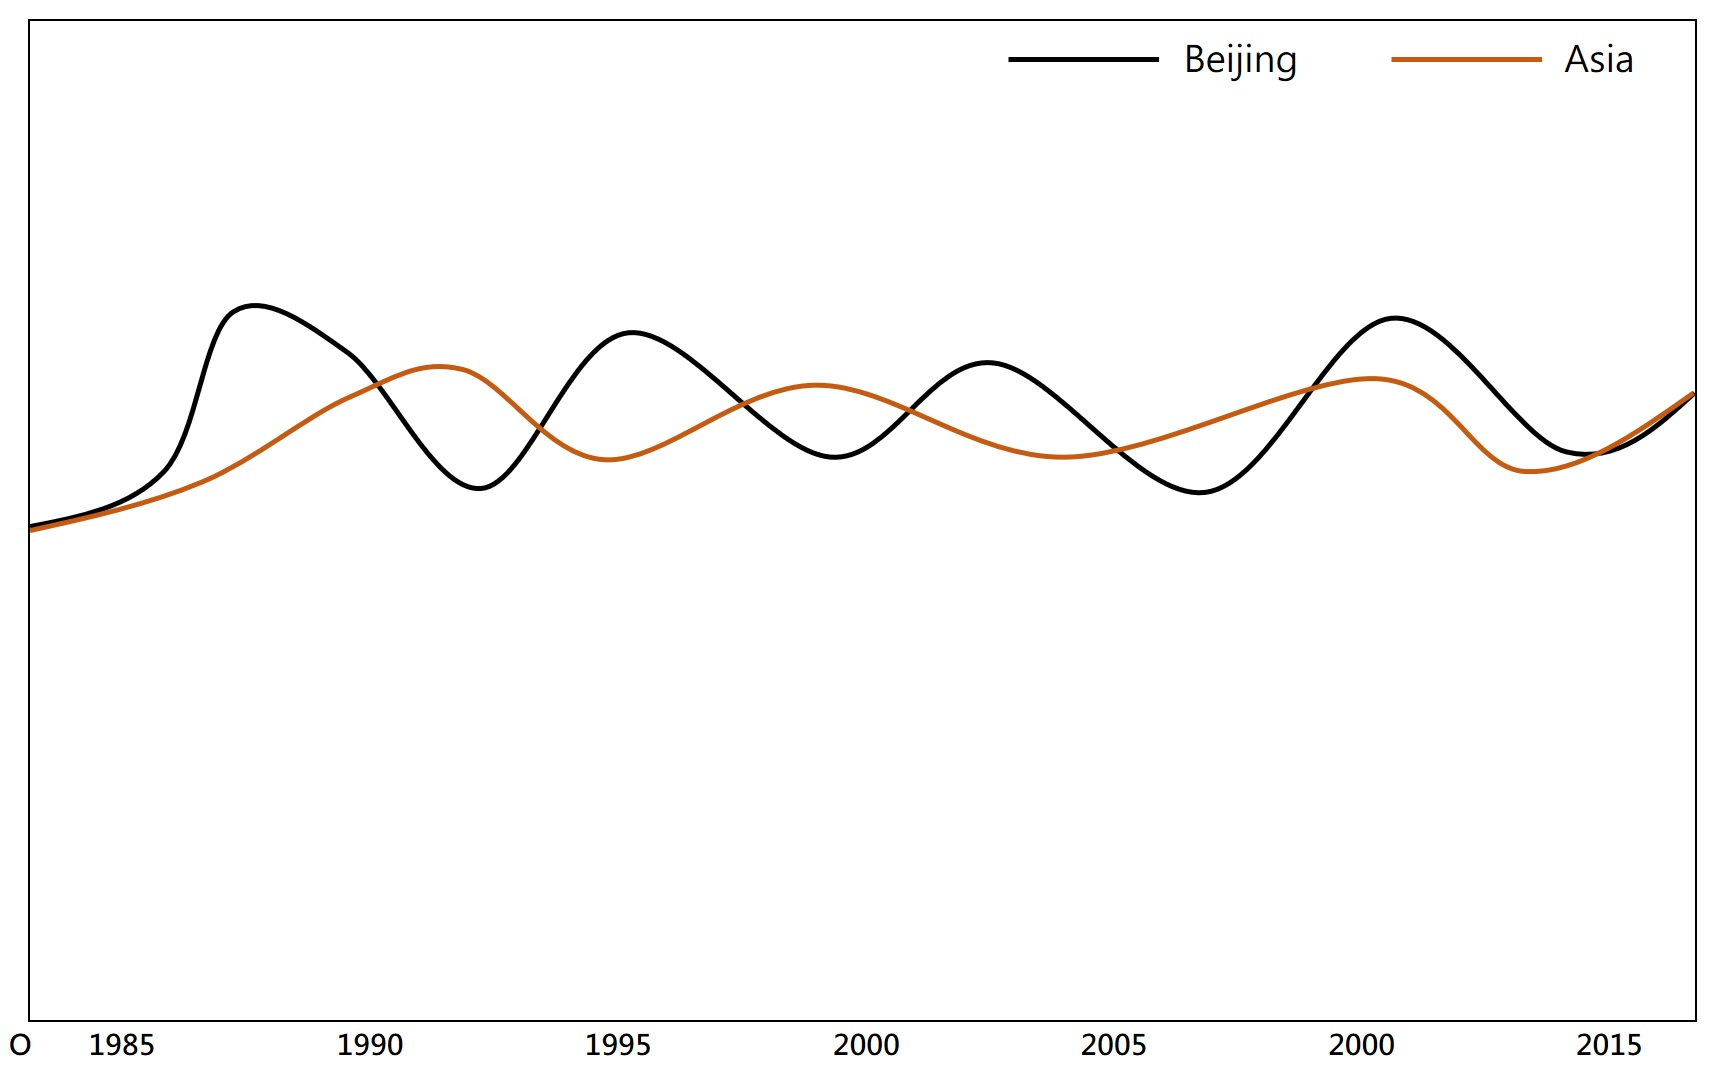
\includegraphics[width=\textwidth]{1.jpg}
\caption{FNI variation trends of Beijing and Asia}
\end{figure}

As is shown in the graph, FNI in city level has more severe fluctuations than FNI in continent level, which is consistent with our assumption. 

\section{Strengths and Weaknesses}
\subsection{Strengths}
\paragraph{Inclusive} Our baseline FNI model and modified FNI model include 20 and 24 independent indicators respectively. These indicators represent most of the major factors that determine the fragility of a "state", making the models relatively reliable and inclusive.
\paragraph{Sufficient Literature Proof} The way Climate Change acts on the indicators is given detailed description according to the literature reference and actual situation, making the models more reliable.
\paragraph{Comprehensive Methods} We take comprehensive utilization of the methods, Analytic Hierarchy Process, Threshold Theory, and Dynamic Programming Algorithm. So our model is convincing and substantial.
\subsection{Weaknesses}
\paragraph{Accuracy Relies on Statistics} In our model, large quantities of statistics are required to ensure the prediction is accurate and reliable. Thus, the FNI model is dependent on the database to guarantee the accuracy.
\paragraph{Reaction to Climate Change Is Not Included} Since the tasks require us to look into the ways how Climate Change influences regional fragility, components' reaction such as economic reaction to Climate Change is not included in our model.

\bibliographystyle{apalike}
\bibliography{icmmcm}

\appendix
\appendixpage
\begin{figure} [H]
\centering
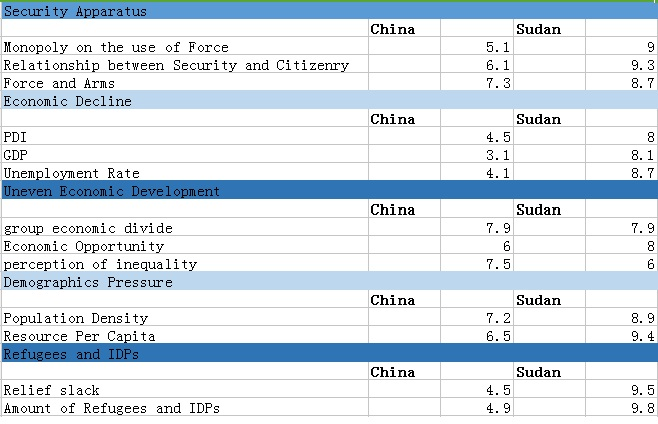
\includegraphics[width=\textwidth]{output3.jpg}
\caption{evaluating criteria for some items}
\end{figure}

\begin{figure} [H]
\centering

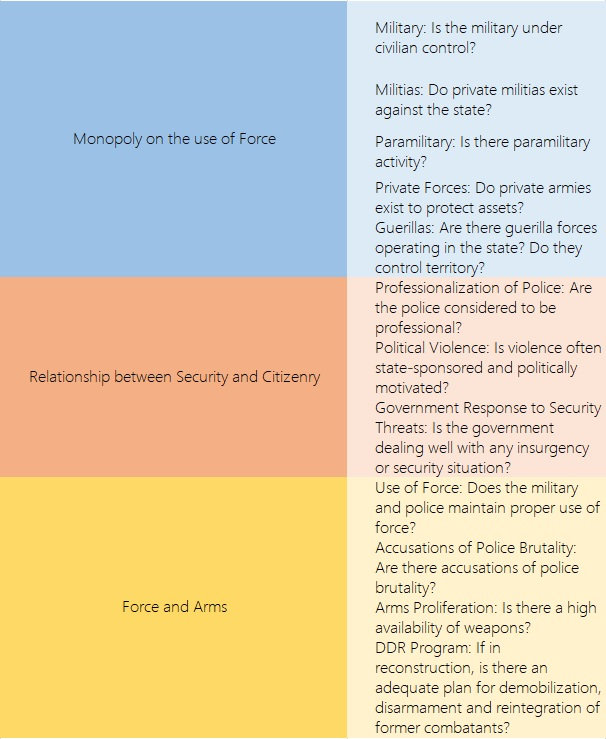
\includegraphics[width=\textwidth]{output2.jpg}
\caption{raw data input for model}
\end{figure}
\label{fig6}
\begin{lstlisting}[language=c++]

The code of Analytic Hierarchy Process in C++

#include<stdio.h>
#include<math.h>
#include<algorithm>
using namespace std;
const int maxn=101;
double val[maxn];
double a[maxn][maxn],b[maxn][maxn];
int N;
void input(){
	for(int i=1;i<=N;i++)
		scanf("%lf",&val[i]);
	for(int i=1;i<=N;i++)
		for(int j=1;j<=N;j++){
			double tmp=fabs(val[i]-val[j]);
			if(tmp<2){
				a[i][j]=1;
				continue;
			}
			if(tmp<4){
				if(val[i]>val[j])a[i][j]=3;
				else a[i][j]=1.0/3.0;
				continue;
			}
			
			if(tmp<6){
				if(val[i]>val[j])a[i][j]=5;
				else a[i][j]=1.0/5.0;
				continue;
			}
			if(tmp<8){
				if(val[i]>val[j])a[i][j]=7;
				else a[i][j]=1.0/7.0;
				continue;
			}
			if(val[i]>val[j])a[i][j]=9;
			else a[i][j]=1.0/9.0;
		}
	for(int i=1;i<=N;i++)
		for(int j=1;j<=N;j++)
			b[i][j]=a[i][j];
}
void SQRT(){
	double minn=1000,maxx=-1000;
	for(int i=1;i<=N;i++){
		for(int j=2;j<=N;j++)
			a[i][1]*=a[i][j];
		a[i][1]=pow(a[i][1],1.0/N);
		minn=min(a[i][1],minn);
		maxx=max(a[i][1],maxx);
	}
	for(int i=1;i<=N;i++){
		printf("%lf ",atan(a[i][1])*2/3.1415926);
	}
	puts("");
}
void SUM(){
	double minn,maxx;
	for(int j=1;j<=N;j++){
		minn=b[1][j];maxx=b[1][j];
		for(int i=2;i<=N;i++){
			minn=min(b[i][j],minn);
			maxx=max(b[i][j],maxx);
		}
		for(int i=1;i<=N;i++){
			b[i][j]=(b[i][j]-minn)/(maxx-minn);
			b[0][j]+=b[i][j];
		}
		printf("%lf ",b[0][j]/N);
	}
	puts("");
}
int main(){
	freopen("input.txt","r",stdin);
	while(scanf("%d",&N)!=EOF)
		input();
	SQRT();
	SUM();
	return 0;
}
\end{lstlisting}
\label{prog}

\end{document}


